\documentclass[11pt,letterpaper]{article}
\PassOptionsToPackage{hyphens}{url}
\usepackage[margin=.83in,top=.8in,bottom=.8in,headheight=15pt]{geometry}
\usepackage[T1]{fontenc}
\usepackage{lmodern,amsmath,amssymb,mathtools,bm,booktabs,array,graphicx,tikz}
\usetikzlibrary{arrows.meta,positioning,calc,decorations.pathreplacing,patterns}
\definecolor{ink}{HTML}{17344D}\definecolor{accent}{HTML}{087E8B}\definecolor{pale}{HTML}{EDF5F5}\definecolor{gold}{HTML}{AD6B19}
\providecommand{\dd}{\,\mathrm{d}}\providecommand{\R}{\mathbb{R}}
\providecommand{\E}{\mathbb{E}}\providecommand{\Var}{\operatorname{Var}}
\providecommand{\Cov}{\operatorname{Cov}}\providecommand{\diag}{\operatorname{diag}}
\providecommand{\norm}[1]{\left\lVert#1\right\rVert}
\providecommand{\abs}[1]{\left|#1\right|}
\usepackage{microtype,hyperref,fancyhdr,enumitem,amsthm,sectsty,needspace}
\allsectionsfont{\raggedright}
\hypersetup{colorlinks=true,linkcolor=ink,urlcolor=accent,pdfauthor={Zan Ahmad},pdftitle={Crossbridge populations: transition kinetics and mechanical force / Lecture notes}}
\setlength{\parindent}{0pt}\setlength{\parskip}{6pt}\linespread{1.07}
\setlist{itemsep=3pt,topsep=4pt,leftmargin=*}
\emergencystretch=2em\clubpenalty=10000\widowpenalty=10000
\pagestyle{fancy}\fancyhf{}\fancyhead[L]{\small Mathematical Modeling}\fancyhead[R]{\small Lecture 5}
\fancyfoot[L]{\footnotesize Zan Ahmad}\fancyfoot[R]{\footnotesize\thepage}\renewcommand{\headrulewidth}{.3pt}
\newtheorem{proposition}{Proposition}\newtheorem{theorem}{Theorem}\newtheorem{lemma}{Lemma}
\theoremstyle{definition}\newtheorem{definition}{Definition}\newtheorem{example}{Example}
\numberwithin{equation}{section}
\begin{document}
{\small\scshape Mathematical Modeling\hfill Lecture 5}\par\medskip
{\raggedright\hyphenpenalty=10000\exhyphenpenalty=10000\LARGE\bfseries\color{ink} Crossbridge populations: transition kinetics and mechanical force\par}\medskip
{\small Lecture notes}\par\bigskip
We derive an occupancy equation from molecular transitions, solve it exactly, and then identify the mechanical information lost by reducing a displacement distribution to one fraction. The synthetic calculation isolates attachment kinetics; it is not a measured force--velocity relation.

\section{A two-state description of crossbridge occupancy}
\hypertarget{note-a-two-state-description-of-crossbridge-occupancy}{}\label{note:a-two-state-description-of-crossbridge-occupancy}
{\small \href{slides.html\#frame=attached-and-detached-populations\&step=1}{Slides for this section}}\par
Actin and myosin filaments slide relative to one another; shortening need not mean that either filament becomes shorter. A myosin head can attach, carry force, and detach. The detailed force depends on its configuration as well as its chemical state. We first retain only whether a head is attached. This defines an occupancy model, whose mechanical interpretation requires an additional assumption.

Let $N$ be a fixed number of heads and let $A(t)$ be the attached fraction. The detached fraction is $D(t)=1-A(t)$, so $A,D\geq0$ and $A+D=1$. The variables may denote probabilities for a representative head or population-average fractions. They are not integer counts. If $N=1000$ and $A=0.25$, the mean attached count is $250$.

Define nonnegative attachment and detachment rate constants $f,g$, in $\mathrm{s}^{-1}$. In a short interval $\Delta t$, a detached head attaches with probability $f\Delta t+o(\Delta t)$; an attached head detaches with probability $g\Delta t+o(\Delta t)$. A rate is not a finite-interval probability. In particular, $f$ can exceed $1\,\mathrm{s}^{-1}$ without violating probability bounds. The fluxes of population fraction are
\[
J_{D\to A}=fD=f(1-A),\qquad J_{A\to D}=gA.
\]
The factors $D$ and $A$ enforce availability of the source population.
\begin{center}\begin{minipage}{.98\linewidth}\centering
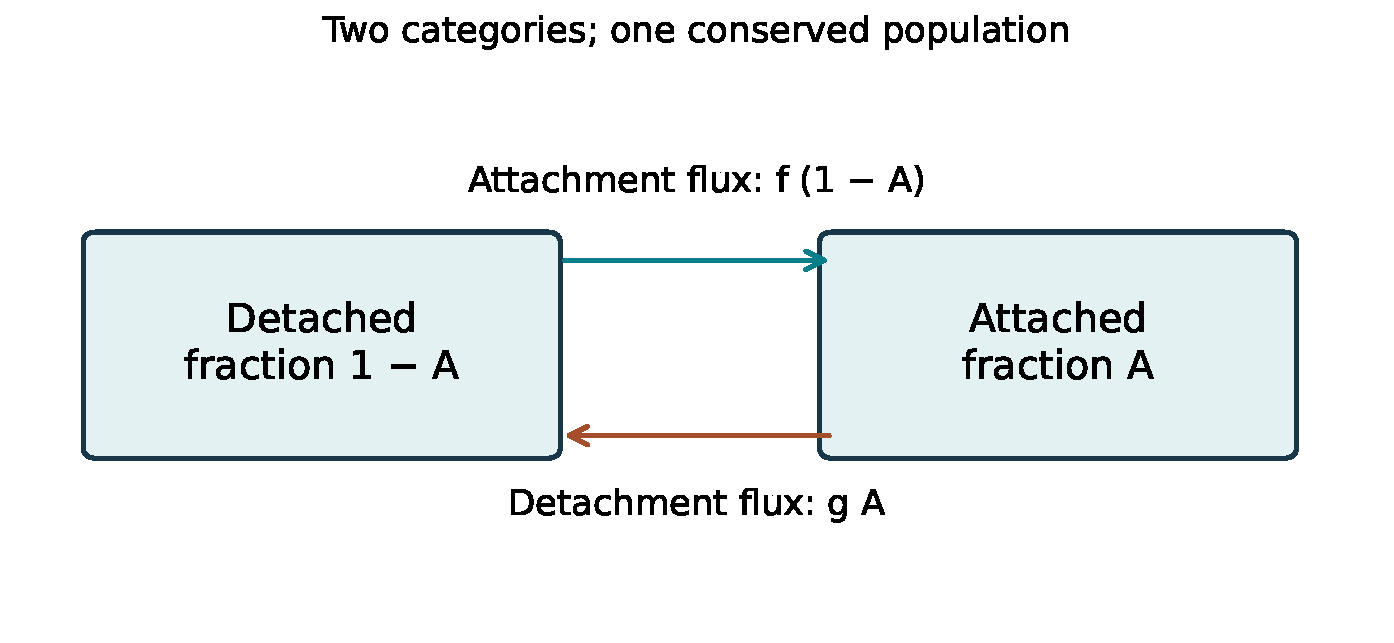
\includegraphics[width=.96\linewidth,height=.57\textheight,keepaspectratio]{state-balance.pdf}\par\smallskip
{\small Original two-state model: every attachment transfers population from detached to attached; detachment transfers it back. Fluxes depend on the available source fraction.}
\end{minipage}\end{center}
\section{Conservation and the transition generator}
\hypertarget{note-conservation-and-the-transition-generator}{}\label{note:conservation-and-the-transition-generator}
{\small \href{slides.html\#frame=transition-fluxes-figure\&step=1}{Slides for this section}}\par
Each transition removes a head from one category and adds it to the other. Therefore
\[
\frac{\dd}{\dd t}\begin{pmatrix}D\\A\end{pmatrix}
=\begin{pmatrix}-f&g\\ f&-g\end{pmatrix}\begin{pmatrix}D\\A\end{pmatrix},
\qquad \frac{\dd}{\dd t}(D+A)=0.
\]
The columns of this matrix sum to zero; its off-diagonal entries are nonnegative. These are the conservation and sign properties of a two-state continuous-time Markov generator in the column-vector convention. Substituting $D=1-A$ leaves one independent state:
\[
\boxed{\dot A=f(1-A)-gA=f-(f+g)A.}
\]
At $A=0$ the derivative is $f\geq0$; at $A=1$ it is $-g\leq0$. Thus the continuous dynamics cannot leave $[0,1]$. For $f=3$, $g=1$, and $A=0.5$, attachment contributes $1.5\,\mathrm{s}^{-1}$ and detachment contributes $0.5\,\mathrm{s}^{-1}$. The net initial slope is $1\,\mathrm{s}^{-1}$. These fluxes describe fractions per second, not the number of cycles completed by every head.
\section{Equilibrium, relaxation, and rate identification}
\hypertarget{note-equilibrium-relaxation-and-rate-identification}{}\label{note:equilibrium-relaxation-and-rate-identification}
{\small \href{slides.html\#frame=equilibrium-with-continuing-turnover\&step=1}{Slides for this section}}\par
Assume $f+g>0$. Equating the fluxes gives
\[
A_\infty=\frac{f}{f+g},\qquad \tau=\frac1{f+g},\qquad
\frac{\dd}{\dd t}(A-A_\infty)=-\frac{A-A_\infty}{\tau}.
\]
Integrating the last equation yields
\[
A(t)=A_\infty+(A_0-A_\infty)e^{-t/\tau}.
\]
This is a convex combination of $A_0$ and $A_\infty$, proving the fraction bound again and showing monotone approach to equilibrium. For $f=g=0$, the equation instead gives $A(t)=A_0$; the ratio $0/0$ must not be evaluated.

With $f=3\,\mathrm{s}^{-1}$ and $g=1\,\mathrm{s}^{-1}$, $A_\infty=0.75$ and $\tau=0.25\,\mathrm{s}$. Both equilibrium fluxes equal $0.75\,\mathrm{s}^{-1}$. A steady fraction therefore permits continuing molecular turnover. Multiplying both rates by $c>0$ leaves $A_\infty$ unchanged and divides $\tau$ by $c$. An endpoint alone identifies only their ratio. If a constant-rate experiment identifies both $A_\infty$ and $\tau$, then
\[
f=\frac{A_\infty}{\tau},\qquad g=\frac{1-A_\infty}{\tau}.
\]
This inference presupposes that the two-state, constant-rate model is appropriate and that the observed quantity actually measures occupancy.
\section{Rate changes and numerical preservation of fractions}
\hypertarget{note-rate-changes-and-numerical-preservation-of-fractions}{}\label{note:rate-changes-and-numerical-preservation-of-fractions}
{\small \href{slides.html\#frame=exact-updates-across-rate-switches\&step=1}{Slides for this section}}\par
At a prescribed rate switch, $A$ remains continuous: a bounded change of rate does not instantaneously move a finite fraction of heads. For each interval of length $h$ with fixed rates, use
\[
A_{n+1}=A_\infty+(A_n-A_\infty)e^{-(f+g)h}.
\]
The final state of one interval is the initial state of the next. In the demonstration, $A_0=0.5$, $g=1\,\mathrm{s}^{-1}$, and $f$ equals $1$, $3$, and $0\,\mathrm{s}^{-1}$ on successive one-second intervals. Thus
\[
A(1)=0.5,\quad A(2)=0.75-0.25e^{-4}\simeq0.74542,
\quad A(3)=A(2)e^{-1}\simeq0.27422.
\]
The slope jumps at each switch, while the state does not.

An Euler approximation gives $A_{n+1}=A_n+h[f(1-A_n)-gA_n]$. At $A_n=0.5$ and $h=0.05\,\mathrm{s}$ the estimate is $0.55$; the exact update is $0.75-0.25e^{-0.2}\simeq0.54532$. The exact formula is preferable for this constant-rate problem. Euler maps the entire interval $[0,1]$ into itself if $hf\leq1$ and $hg\leq1$: check its affine map at the two endpoints. The stronger condition $h(f+g)\leq1$ also makes approach to equilibrium nonoscillatory. Neither bound substitutes for an accuracy study. Clipping an invalid fraction conceals an error in the numerical update.
\begin{center}\begin{minipage}{.98\linewidth}\centering
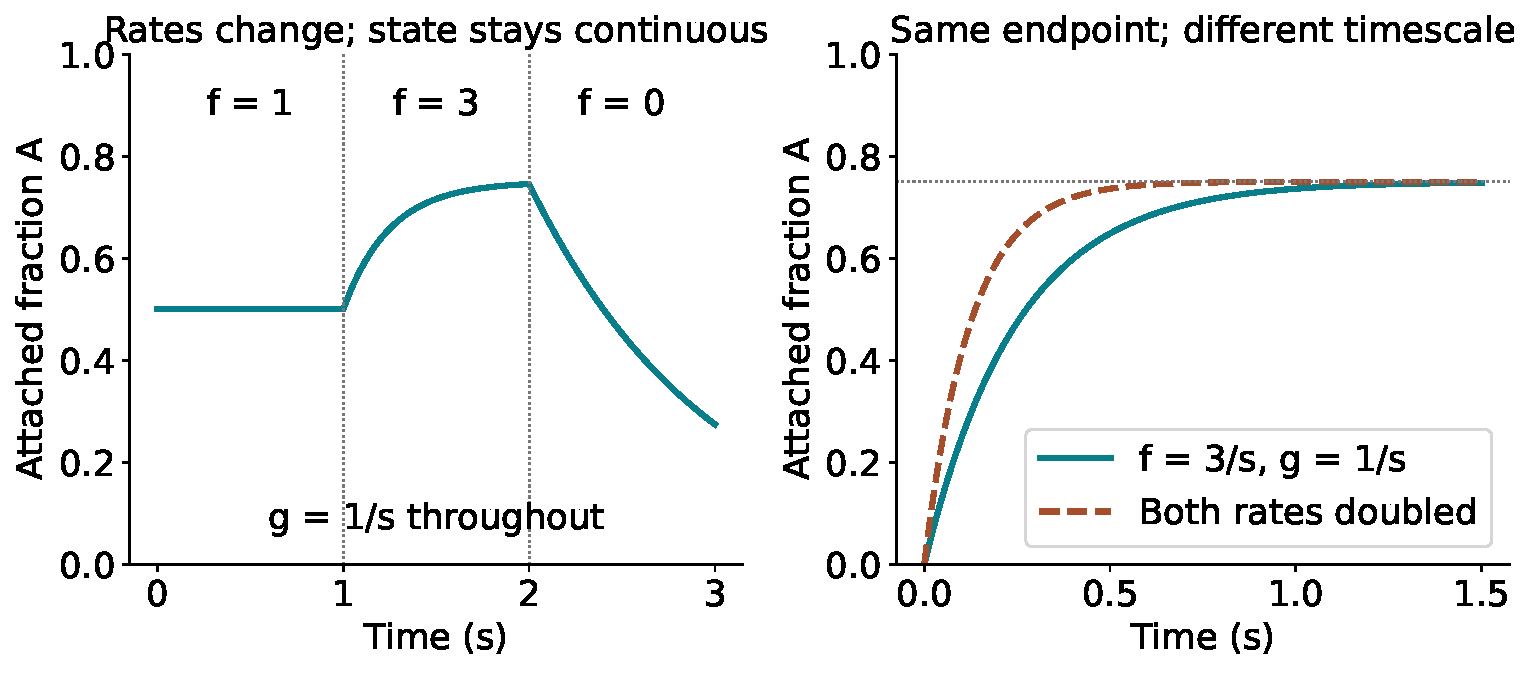
\includegraphics[width=.96\linewidth,height=.57\textheight,keepaspectratio]{occupancy-traces.pdf}\par\smallskip
{\small Synthetic exact trajectories. Left: attachment rate changes from 1 to 3 to 0 per second while detachment remains 1 per second. Right: doubling both rates preserves equilibrium 0.75 and halves the timescale.}
\end{minipage}\end{center}
\section{Mechanical force requires a distribution or a closure}
\hypertarget{note-mechanical-force-requires-a-distribution-or-a-closure}{}\label{note:mechanical-force-requires-a-distribution-or-a-closure}
{\small \href{slides.html\#frame=a-fixed-force-closure\&step=1}{Slides for this section}}\par
If every attached head contributes the same aligned force $F_{\mathrm{head}}$, the total force is
\[
F=N A F_{\mathrm{head}}.
\]
For $N=1000$, $A=0.75$, and $F_{\mathrm{head}}=2\,\mathrm{pN}$, this gives $1500\,\mathrm{pN}=1.5\,\mathrm{nN}$. It is a separate constitutive closure, not a consequence of occupancy balance.

To see the information it discards, let $u(x,t)\dd x$ be the fraction of heads attached with displacement in $[x,x+\dd x]$. Then
\[
A(t)=\int_{\R}u(x,t)\,\dd x,\qquad
F(t)=N\int_{\R}p(x)u(x,t)\,\dd x.
\]
Here $u$ has units of inverse length and $p(x)$ is the force of one head. With $p(x)=\kappa x$, force depends on the first displacement moment; occupancy is the zeroth moment. Equal occupancy does not imply equal force. For example, populations concentrated at $x_1$ and $x_2$ with the same attached fraction have forces $NA\kappa x_1$ and $NA\kappa x_2$.

For a spatially uniform shortening velocity $v(t)$, a density description may take the form
\[
\partial_tu-v\partial_xu=f(1-A)\delta(x-x_a)-g u.
\]
If $u$ decays at both ends and $g$ is independent of displacement, integrating recovers $\dot A=f(1-A)-gA$. The transport term vanishes in this zeroth-moment balance, but remains relevant to force. This connection explains why a valid occupancy reduction still cannot derive a force--velocity curve.
\Needspace{10\baselineskip}
\section{Computation and the scope of a force measurement}
\hypertarget{note-computation-and-the-scope-of-a-force-measurement}{}\label{note:computation-and-the-scope-of-a-force-measurement}
{\small \href{slides.html\#frame=rate-experiments-in-the-companion\&step=1}{Slides for this section}}\par
The supplied program evaluates exact constant-rate intervals and draws synthetic trajectories. Its checks include interval composition, pure detachment, zero rates, fraction bounds, and equivalence between doubling rates and doubling elapsed time. These checks assess the implementation of the stated model. They do not establish that real crossbridges have configuration-independent rates.

In the notebook, compare $(f,g)=(3,1)$ with $(6,2)$ at equal physical times and then at rescaled times. Record both the endpoint and the time constant. Changing $N$ changes the fixed-force readout but leaves occupancy dynamics unchanged; changing $F_{\mathrm{head}}$ does the same. A force trace alone therefore cannot uniquely separate occupancy, population size, and per-head mechanics without further observations.

Finally, mechanical power $Fv$ and chemical power are distinct. At zero shortening speed, mechanical power is zero even while attachment and detachment continue. ATP use and chemical free-energy consumption require additional stoichiometry and energetic assumptions. Neither a force curve nor the two occupancy fluxes alone supplies those quantities.
\bigskip
\section*{Exercises}
\par\noindent\begin{minipage}{\linewidth}
\subsection*{MM05-E1. Account for both directions}
Use A =\allowbreak{} 0.2, f =\allowbreak{} 2/s and g =\allowbreak{} 3/s.

\textbf{a} Compute attachment, detachment and net flux with units.

\end{minipage}\par\medskip
\textbf{b} Estimate A after 0.05 s using the starting net flux. Explain why this is an estimate.

\textbf{c} Find the equilibrium and determine whether the initial fraction moves toward it.

\par\noindent\begin{minipage}{\linewidth}
\subsection*{MM05-E2. Separate endpoint from speed}
Compare f =\allowbreak{} 4/s, g =\allowbreak{} 2/s with f =\allowbreak{} 8/s, g =\allowbreak{} 4/s.

\textbf{a} Compute both equilibrium fractions.

\end{minipage}\par\medskip
\textbf{b} Compute both relaxation times and compare them.

\textbf{c} Can an equilibrium fraction alone distinguish these models? Propose an observation that can.

\par\noindent\begin{minipage}{\linewidth}
\subsection*{MM05-E3. Check a force readout}
Assume 800 heads, attached fraction 0.6 and an aligned force of 3 pN per attached head.

\textbf{a} Compute the average attached count and total force.

\end{minipage}\par\medskip
\textbf{b} If the head population doubles while the fraction and per-head force stay fixed, what changes?

\textbf{c} Explain why this calculation cannot predict shortening speed or ATP power.

\par\noindent\begin{minipage}{\linewidth}
\subsection*{MM05-E4. Use limiting cases to challenge code}
A proposed implementation should preserve attached fractions between zero and one.

\textbf{a} Predict the trajectory when both rates are zero and A0 =\allowbreak{} 0.3.

\end{minipage}\par\medskip
\textbf{b} Predict the direction and endpoint when f =\allowbreak{} 0, g > 0 and A0 > 0.

\textbf{c} A large explicit step gives A =\allowbreak{} 1.2. Explain what failed and how to investigate without silently clipping.

\section*{References}
\noindent\begin{minipage}{\linewidth}
Zan Ahmad, Fall 2024 HEART syllabus. PDF pages 1--2.

\end{minipage}\par\medskip
\noindent\begin{minipage}{\linewidth}
Hoppensteadt and Peskin, Modeling and Simulation in Medicine and the Life Sciences, second edition. Printed pages 171--175; PDF pages 184--188 in the supplied copy.

\end{minipage}\par\medskip
\end{document}
